These plots show a second-order Markov model for the turning behavior. These models answer the question of whether the $k$-th saccade direction depends also on the $(k-2)$-th saccade direction as well as the $(k-1)-th$. 

Each model has 4 states, labeled `LL',  `LR', `RL', `RR'. `LL' means that the last two saccades were both left, `LR' means that the next-to-last was left and the last right, and so on. Each state has still 2 transitions (`left' and `right'). For example, the transition `left' leads from  `LR' to `RL'.

The plots show that the next-to-last state helps predicting the next direction. If this wasn't the case, then the states \{`LL', `RL'\} and \{`LR', `RR'\} would be equivalent (that is, having the same transition probabilities).
This shows that, assuming all this behavior comes from internal random timers, there is no clear `reset' mechanism that makes forget the history when we a saccade is initiated. 

The analysis on the free-flying data showed a different result: while the last saccade helps in predicting the next, the next-to-last does not (the states \{`LL', `RL'\} and \{`LR', `RR'\} were indeed equivalent).

The equivalent data for  \Dmelanogaster in free-flight  are shown in Fig.~\vref{fig:ff-markov_second}.

\vfill
\begin{figure}[h!]
	\centering
	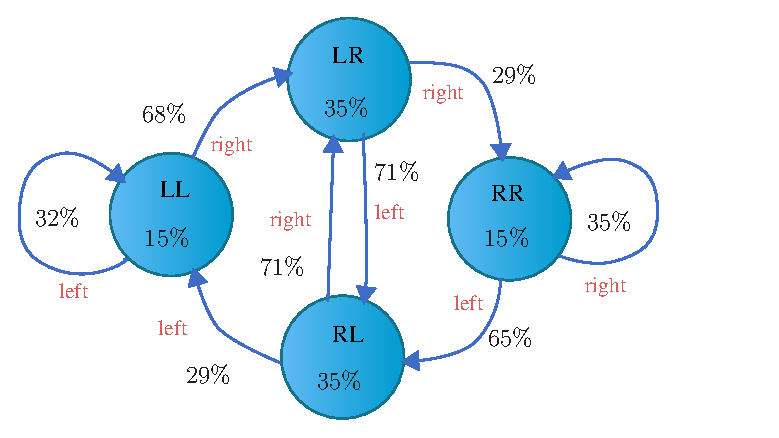
\includegraphics[width=6cm]{../comments/freeflight/markov_second}
	\caption{ \label{fig:ff-markov_second}   \Dmelanogaster (Mamarama) }
\end{figure}